\documentclass[border=8pt]{standalone}
\usepackage{tikz}
\usetikzlibrary{arrows.meta}

\definecolor{wallTop}{HTML}{EAF1F8}
\definecolor{wallBase}{HTML}{D6E1EC}
\definecolor{baseboard}{HTML}{C3CEDA}
\definecolor{floorA}{HTML}{CFA271}
\definecolor{floorB}{HTML}{BE8E58}
\definecolor{floorLine}{HTML}{A97B47}
\definecolor{rugA}{HTML}{9FCFB4}
\definecolor{rugB}{HTML}{86BEA1}
\definecolor{woodA}{HTML}{A9713F}
\definecolor{woodB}{HTML}{8A5A31}
\definecolor{woodC}{HTML}{6E4626}
\definecolor{doorFrameC}{HTML}{B99B6B}
\definecolor{doorSlab}{HTML}{E3D2B4}
\definecolor{hallDark}{HTML}{2E2C36}
\definecolor{screenDark}{HTML}{263445}
\definecolor{screenGlow}{HTML}{4A7FA8}
\definecolor{metalGray}{HTML}{9AA7B1}
\definecolor{skin}{HTML}{F6D2B4}
\definecolor{skinDark}{HTML}{E0B392}
\definecolor{blush}{HTML}{F2A6A0}
\definecolor{hairSon}{HTML}{3B2E2A}
\definecolor{hairMom}{HTML}{4B3A33}
\definecolor{shirtSon}{HTML}{4CA3DD}
\definecolor{shirtSonDark}{HTML}{3A87BC}
\definecolor{pantsSon}{HTML}{3B4A63}
\definecolor{shoeSon}{HTML}{2C3542}
\definecolor{blouseMom}{HTML}{B5838D}
\definecolor{blouseMomDark}{HTML}{9C6C76}
\definecolor{apronMom}{HTML}{F4EADC}
\definecolor{skirtMom}{HTML}{6D6875}
\definecolor{goggle}{HTML}{2E3440}
\definecolor{goggleLite}{HTML}{6FD3F5}
\definecolor{ctrlBody}{HTML}{37474F}
\definecolor{ctrlRing}{HTML}{90A4AE}
\definecolor{bedFrame}{HTML}{9C6B3E}
\definecolor{blanket}{HTML}{7FA9D6}
\definecolor{blanketDark}{HTML}{6892C0}
\definecolor{sheetWhite}{HTML}{FAFBFD}
\definecolor{bookA}{HTML}{D9705E}
\definecolor{bookB}{HTML}{E8B84B}
\definecolor{bookC}{HTML}{6FA8A0}
\definecolor{bookD}{HTML}{8A79B8}
\definecolor{plantG}{HTML}{6FA86B}
\definecolor{potC}{HTML}{D08B62}
\definecolor{bubbleFill}{HTML}{F3FAFF}
\definecolor{bubbleEdge}{HTML}{8FC6E8}
\definecolor{starY}{HTML}{FFD166}
\definecolor{cubeA}{HTML}{7FD1E8}
\definecolor{cubeB}{HTML}{55B4D4}
\definecolor{cubeC}{HTML}{3E93B2}
\definecolor{gazeC}{HTML}{D2603A}
\definecolor{gazeSon}{HTML}{4C9AC4}
\definecolor{inkC}{HTML}{2B2B33}
\definecolor{motionC}{HTML}{F2A03D}
\definecolor{sweatC}{HTML}{7FC4E8}

\begin{document}
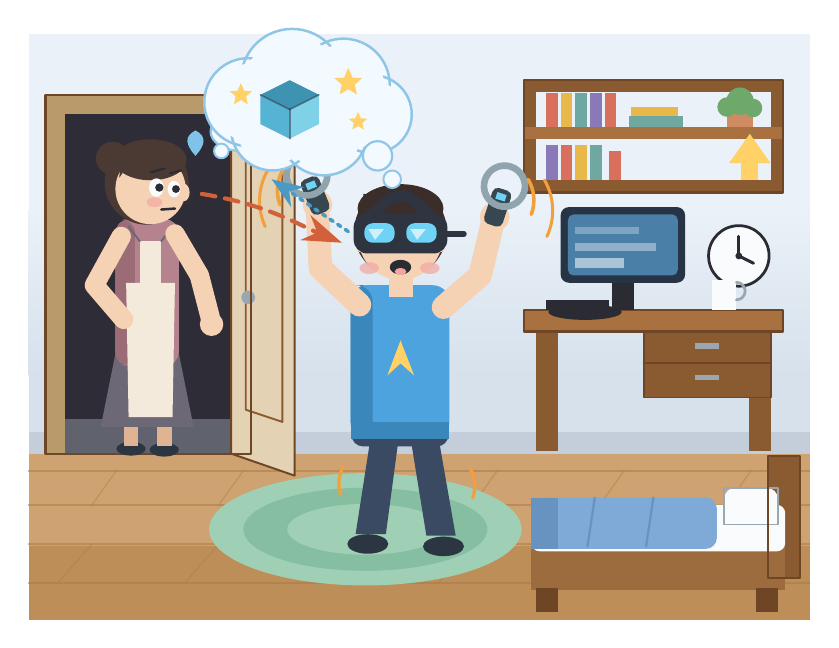
\begin{tikzpicture}[x=0.62cm,y=0.62cm,line join=round,line cap=round]

% ---------- room shell ----------
\fill[wallTop] (0,3.4) rectangle (16,12);
\fill[wallBase] (0,3.4) rectangle (16,6.6);
\shade[top color=wallTop,bottom color=wallBase] (0,5.0) rectangle (16,8.4);
\fill[baseboard] (0,3.4) rectangle (16,3.85);
\fill[floorA] (0,0) rectangle (16,3.4);
\fill[floorB] (0,0) rectangle (16,1.5);
\foreach \y in {0.75,1.55,2.35,3.05}{\draw[floorLine,line width=0.6pt,opacity=0.55] (0,\y) -- (16,\y);}
\foreach \p in {1.3,3.9,6.5,9.1,11.7,14.3}{\draw[floorLine,line width=0.5pt,opacity=0.4] (\p,2.35) -- (\p+0.5,3.05);}
\foreach \p in {0.6,3.2,5.8,8.4,11.0,13.6}{\draw[floorLine,line width=0.5pt,opacity=0.4] (\p,0.75) -- (\p+0.7,1.55);}

% ---------- doorway (left) ----------
\fill[doorFrameC] (0.35,3.4) rectangle (4.55,10.75);
\fill[hallDark] (0.75,3.4) rectangle (4.15,10.35);
\fill[hallDark!70!wallBase] (0.75,3.4) rectangle (4.15,4.1);
\fill[doorSlab] (4.15,3.4) -- (5.45,2.95) -- (5.45,10.05) -- (4.15,10.35) -- cycle;
\draw[woodC,line width=0.7pt] (4.15,3.4) -- (5.45,2.95) -- (5.45,10.05) -- (4.15,10.35) -- cycle;
\draw[woodB,line width=0.7pt] (4.45,4.3) -- (5.2,4.05) -- (5.2,9.3) -- (4.45,9.5) -- cycle;
\fill[metalGray] (4.5,6.6) circle (0.14);
\draw[woodC,line width=0.8pt] (0.35,3.4) rectangle (4.55,10.75);

% ---------- shelf on right wall ----------
\fill[woodB] (10.15,8.75) rectangle (15.45,11.05);
\fill[wallTop] (10.4,9.0) rectangle (15.2,10.8);
\fill[woodA] (10.15,9.85) rectangle (15.45,10.1);
\foreach \x/\c in {10.6/bookA,10.9/bookB,11.2/bookC,11.5/bookD,11.8/bookA}{%
  \fill[\c] (\x,10.1) rectangle (\x+0.24,10.78);}
\fill[bookC] (12.3,10.1) rectangle (13.4,10.32);
\fill[bookB] (12.35,10.32) rectangle (13.3,10.5);
\fill[potC] (14.3,10.1) rectangle (14.85,10.42);
\fill[plantG] (14.575,10.62) circle (0.28);
\fill[plantG] (14.31,10.5) circle (0.2);
\fill[plantG] (14.84,10.48) circle (0.19);
\foreach \x/\c in {10.6/bookD,10.9/bookA,11.2/bookB,11.5/bookC}{%
  \fill[\c] (\x,9.0) rectangle (\x+0.24,9.72);}
\fill[bookA] (11.9,9.0) rectangle (12.14,9.6);
\fill[starY] (14.6,9.0) rectangle (14.95,9.35);
\fill[starY] (14.35,9.35) -- (15.2,9.35) -- (14.775,9.95) -- cycle;
\draw[woodC,line width=0.8pt] (10.15,8.75) rectangle (15.45,11.05);

% ---------- wall clock ----------
\fill[sheetWhite] (14.55,7.45) circle (0.62);
\draw[inkC,line width=1pt] (14.55,7.45) circle (0.62);
\draw[inkC,line width=1.1pt] (14.55,7.45) -- (14.55,7.85);
\draw[inkC,line width=1.1pt] (14.55,7.45) -- (14.85,7.3);
\fill[inkC] (14.55,7.45) circle (0.07);

% ---------- desk ----------
\fill[woodA] (10.15,5.9) rectangle (15.45,6.35);
\fill[woodB] (10.4,3.45) rectangle (10.85,5.9);
\fill[woodB] (14.75,3.45) rectangle (15.2,5.9);
\fill[woodB] (12.6,4.55) rectangle (15.2,5.9);
\draw[woodC,line width=0.7pt] (12.6,4.55) rectangle (15.2,5.9);
\draw[woodC,line width=0.7pt] (12.6,5.25) -- (15.2,5.25);
\fill[metalGray] (13.65,4.9) rectangle (14.15,5.02);
\fill[metalGray] (13.65,5.55) rectangle (14.15,5.67);
\draw[woodC,line width=0.8pt] (10.15,5.9) rectangle (15.45,6.35);

% monitor + keyboard on desk
\fill[inkC] (11.95,6.35) rectangle (12.4,6.95);
\fill[inkC] (11.4,6.3) ellipse (0.75 and 0.16);
\fill[screenDark,rounded corners=3pt] (10.9,6.9) rectangle (13.45,8.45);
\fill[screenGlow,rounded corners=2pt] (11.05,7.05) rectangle (13.3,8.3);
\fill[sheetWhite,opacity=0.55] (11.2,7.2) rectangle (12.2,7.4);
\fill[sheetWhite,opacity=0.4] (11.2,7.55) rectangle (12.85,7.72);
\fill[sheetWhite,opacity=0.3] (11.2,7.9) rectangle (12.5,8.05);
\fill[inkC] (10.6,6.35) rectangle (11.9,6.55);
\fill[sheetWhite] (14.0,6.35) rectangle (14.5,6.95);
\draw[metalGray,line width=1pt] (14.5,6.55) arc (-90:90:0.18);

% ---------- rug ----------
\fill[rugA] (6.9,1.85) ellipse (3.2 and 1.15);
\fill[rugB] (6.9,1.85) ellipse (2.5 and 0.85);
\fill[rugA] (6.9,1.85) ellipse (1.6 and 0.52);

% ---------- bed (right, foreground) ----------
\fill[woodB] (15.15,0.85) rectangle (15.8,3.35);
\fill[bedFrame] (10.3,0.6) rectangle (15.5,1.5);
\fill[woodC] (10.4,0.15) rectangle (10.85,0.65);
\fill[woodC] (14.9,0.15) rectangle (15.35,0.65);
\fill[sheetWhite,rounded corners=3pt] (10.3,1.4) rectangle (15.5,2.35);
\fill[blanket,rounded corners=4pt] (10.3,1.45) rectangle (14.1,2.5);
\fill[blanketDark] (10.3,1.45) rectangle (10.85,2.5);
\draw[blanketDark,line width=0.8pt] (11.6,2.5) -- (11.45,1.5);
\draw[blanketDark,line width=0.8pt] (12.8,2.5) -- (12.65,1.5);
\fill[sheetWhite,rounded corners=4pt] (14.25,1.95) rectangle (15.35,2.7);
\draw[metalGray,line width=0.6pt] (14.25,1.95) rectangle (15.35,2.7);
\draw[woodC,line width=0.8pt] (15.15,0.85) rectangle (15.8,3.35);

% ---------- mother in the doorway ----------
\fill[shoeSon] (2.1,3.5) ellipse (0.3 and 0.14);
\fill[shoeSon] (2.78,3.48) ellipse (0.3 and 0.14);
\fill[skinDark] (1.95,3.55) rectangle (2.25,4.05);
\fill[skinDark] (2.63,3.55) rectangle (2.93,4.05);
\fill[skirtMom] (1.78,5.45) -- (3.08,5.45) -- (3.38,3.95) -- (1.48,3.95) -- cycle;
\fill[blouseMom,rounded corners=5pt] (1.78,5.2) rectangle (3.08,8.2);
\fill[blouseMomDark,rounded corners=5pt] (1.78,5.2) rectangle (2.18,8.2);
\fill[apronMom] (2.05,4.15) -- (2.95,4.15) -- (3.0,6.9) -- (2.0,6.9) -- cycle;
\fill[apronMom] (2.28,6.9) rectangle (2.72,7.75);
\draw[skirtMom,line width=0.7pt] (2.28,7.75) -- (2.05,8.05);
\draw[skirtMom,line width=0.7pt] (2.72,7.75) -- (2.95,8.05);
% arms: one on hip, one on the door frame
\draw[skin,line width=7pt] (1.9,7.85) -- (1.35,6.85) -- (1.95,6.15);
\draw[skin,line width=7pt] (3.0,7.9) -- (3.5,7.05) -- (3.72,6.2);
\fill[skin] (3.75,6.05) circle (0.24);
% head
\fill[hairMom] (2.42,8.95) circle (0.86);
\fill[hairMom] (1.72,9.45) circle (0.34);
\fill[skin] (2.5,8.82) circle (0.72);
\fill[hairMom] (2.5,9.42) ellipse (0.74 and 0.42);
\fill[hairMom] (1.86,9.05) -- (2.2,9.55) -- (1.9,9.6) -- cycle;
\fill[skin] (3.18,8.75) ellipse (0.12 and 0.18);
\fill[sheetWhite] (2.62,8.85) ellipse (0.15 and 0.19);
\fill[sheetWhite] (2.98,8.82) ellipse (0.13 and 0.17);
\fill[inkC] (2.68,8.85) circle (0.085);
\fill[inkC] (3.02,8.82) circle (0.08);
\draw[inkC,line width=0.8pt] (2.5,9.16) -- (2.78,9.24);
\draw[inkC,line width=0.8pt] (2.9,9.14) -- (3.12,9.2);
\draw[inkC,line width=0.9pt] (2.72,8.4) -- (3.0,8.42);
\fill[blush,opacity=0.65] (2.58,8.55) ellipse (0.16 and 0.1);
% sweat drop
\fill[sweatC] (3.42,9.5) .. controls (3.62,9.72) and (3.66,9.9) .. (3.42,10.02)
  .. controls (3.18,9.9) and (3.22,9.72) .. (3.42,9.5) -- cycle;
% small "..." bubble
\fill[bubbleFill] (4.35,10.0) ellipse (0.62 and 0.4);
\draw[bubbleEdge,line width=0.8pt] (4.35,10.0) ellipse (0.62 and 0.4);
\fill[bubbleFill] (3.95,9.6) circle (0.15);
\draw[bubbleEdge,line width=0.7pt] (3.95,9.6) circle (0.15);
\foreach \x in {4.08,4.35,4.62}{\fill[inkC] (\x,10.0) circle (0.075);}

% ---------- son playing VR ----------
\fill[shoeSon] (6.95,1.55) ellipse (0.42 and 0.2);
\fill[shoeSon] (8.5,1.5) ellipse (0.42 and 0.2);
\fill[pantsSon] (7.05,4.0) -- (7.62,4.0) -- (7.32,1.75) -- (6.7,1.75) -- cycle;
\fill[pantsSon] (7.78,4.0) -- (8.35,4.0) -- (8.75,1.72) -- (8.15,1.72) -- cycle;
\fill[pantsSon,rounded corners=4pt] (6.62,3.55) rectangle (8.6,4.35);
\fill[shirtSon,rounded corners=6pt] (6.6,3.7) rectangle (8.62,6.85);
\fill[shirtSonDark,rounded corners=6pt] (6.6,3.7) rectangle (7.05,6.85);
\fill[shirtSonDark] (6.6,3.7) rectangle (8.62,4.05);
\fill[starY] (7.35,5.0) -- (7.62,5.72) -- (7.9,5.0) -- (7.62,5.25) -- cycle;
\fill[skin] (7.38,6.6) rectangle (7.88,7.15);
% arms up, holding controllers
\draw[skin,line width=8.5pt] (6.78,6.45) -- (5.98,7.2) -- (5.92,8.35);
\draw[skin,line width=8.5pt] (8.5,6.4) -- (9.25,7.05) -- (9.5,8.1);
\fill[skin] (5.92,8.5) circle (0.3);
\fill[skin] (9.55,8.25) circle (0.3);
% head with hair
\fill[hairSon] (7.62,7.95) circle (0.95);
\fill[skin] (7.62,7.82) circle (0.86);
\fill[hairSon] (7.62,8.42) ellipse (0.88 and 0.5);
\fill[hairSon] (6.82,8.05) -- (7.25,8.7) -- (6.86,8.72) -- cycle;
\fill[skin] (8.42,7.72) ellipse (0.13 and 0.2);
\fill[skin] (6.82,7.72) ellipse (0.13 and 0.2);
% goggles + strap
\draw[goggle,line width=4pt] (6.78,8.02) .. controls (7.62,8.9) .. (8.46,8.02);
\fill[goggle,rounded corners=5pt] (6.66,7.5) rectangle (8.58,8.32);
\fill[goggleLite,rounded corners=3pt] (6.88,7.72) rectangle (7.5,8.12);
\fill[goggleLite,rounded corners=3pt] (7.74,7.72) rectangle (8.36,8.12);
\fill[sheetWhite,opacity=0.7] (6.96,8.0) -- (7.28,8.0) -- (7.1,7.78) -- cycle;
\fill[sheetWhite,opacity=0.7] (7.82,8.0) -- (8.14,8.0) -- (7.96,7.78) -- cycle;
\draw[goggle,line width=2pt] (8.58,7.9) -- (8.92,7.9);
% happy open mouth + blush
\fill[blush,opacity=0.7] (6.98,7.2) ellipse (0.2 and 0.12);
\fill[blush,opacity=0.7] (8.22,7.2) ellipse (0.2 and 0.12);
\fill[inkC] (7.62,7.22) ellipse (0.22 and 0.15);
\fill[blush] (7.62,7.13) ellipse (0.12 and 0.07);
% controllers
\begin{scope}[shift={(5.86,8.72)},rotate=22]
  \fill[ctrlBody,rounded corners=2pt] (-0.2,-0.42) rectangle (0.2,0.35);
  \draw[ctrlRing,line width=2.4pt] (0,0.42) circle (0.42);
  \fill[goggleLite] (-0.1,0.12) rectangle (0.1,0.26);
\end{scope}
\begin{scope}[shift={(9.62,8.48)},rotate=-18]
  \fill[ctrlBody,rounded corners=2pt] (-0.2,-0.42) rectangle (0.2,0.35);
  \draw[ctrlRing,line width=2.4pt] (0,0.42) circle (0.42);
  \fill[goggleLite] (-0.1,0.12) rectangle (0.1,0.26);
\end{scope}
% motion arcs
\draw[motionC,line width=1.3pt] (5.15,8.5) arc (200:150:0.85);
\draw[motionC,line width=1.1pt] (4.85,8.05) arc (205:150:1.25);
\draw[motionC,line width=1.3pt] (10.3,8.3) arc (-20:30:0.85);
\draw[motionC,line width=1.1pt] (10.62,7.85) arc (-25:30:1.25);
\draw[motionC,line width=1.2pt] (6.4,2.55) arc (200:150:0.7);
\draw[motionC,line width=1.2pt] (9.1,2.5) arc (-20:30:0.7);

% ---------- VR imagination bubble ----------
\foreach \c/\r in {{(4.5,10.6)}/0.9,{(5.4,11.05)}/1.05,{(6.45,10.95)}/0.95,
                   {(7.05,10.35)}/0.8,{(5.0,10.05)}/0.85,{(6.05,10.0)}/0.9}{%
  \fill[bubbleFill] \c circle (\r);}
\foreach \c/\r in {{(4.5,10.6)}/0.9,{(5.4,11.05)}/1.05,{(6.45,10.95)}/0.95,
                   {(7.05,10.35)}/0.8,{(5.0,10.05)}/0.85,{(6.05,10.0)}/0.9}{%
  \draw[bubbleEdge,line width=0.9pt] \c circle (\r);}
\foreach \c/\r in {{(4.5,10.6)}/0.78,{(5.4,11.05)}/0.93,{(6.45,10.95)}/0.83,
                   {(7.05,10.35)}/0.68,{(5.0,10.05)}/0.73,{(6.05,10.0)}/0.78}{%
  \fill[bubbleFill] \c circle (\r);}
% floating cube inside the bubble
\fill[cubeA] (5.35,10.45) -- (5.95,10.75) -- (5.95,10.15) -- (5.35,9.85) -- cycle;
\fill[cubeB] (5.35,10.45) -- (4.75,10.75) -- (4.75,10.15) -- (5.35,9.85) -- cycle;
\fill[cubeC] (5.35,10.45) -- (5.95,10.75) -- (5.35,11.05) -- (4.75,10.75) -- cycle;
\draw[inkC,line width=0.6pt,opacity=0.5] (5.35,10.45) -- (5.95,10.75);
\draw[inkC,line width=0.6pt,opacity=0.5] (5.35,10.45) -- (4.75,10.75);
\draw[inkC,line width=0.6pt,opacity=0.5] (5.35,10.45) -- (5.35,9.85);
% stars
\foreach \px/\py/\s in {6.55/11.0/0.3,4.35/10.75/0.24,6.75/10.2/0.2}{%
  \begin{scope}[shift={(\px,\py)},scale=\s]
    \fill[starY] (0,1) -- (0.29,0.34) -- (0.95,0.31) -- (0.45,-0.14)
      -- (0.59,-0.81) -- (0,-0.45) -- (-0.59,-0.81) -- (-0.45,-0.14)
      -- (-0.95,0.31) -- (-0.29,0.34) -- cycle;
  \end{scope}}
% bubble tail
\fill[bubbleFill] (7.15,9.5) circle (0.3);
\draw[bubbleEdge,line width=0.8pt] (7.15,9.5) circle (0.3);
\fill[bubbleFill] (7.45,9.02) circle (0.18);
\draw[bubbleEdge,line width=0.7pt] (7.45,9.02) circle (0.18);

% ---------- gaze relations ----------
\draw[gazeC,line width=1.5pt,dashed,dash pattern=on 5pt off 3.5pt,-{Stealth[length=5mm,width=3.4mm]}]
  (3.55,8.72) .. controls (4.9,8.5) and (5.5,8.1) .. (6.42,7.72);
\draw[gazeSon,line width=1.3pt,dotted,-{Stealth[length=4mm,width=3mm]}]
  (6.55,7.95) .. controls (5.95,8.35) and (5.45,8.7) .. (4.98,9.02);

\end{tikzpicture}
\end{document}
